\documentclass[a4paper,11pt]{article}
\usepackage[utf8]{inputenc}
\usepackage{polski}
\usepackage{graphicx}
\usepackage[left=1in,right=1in]{geometry}
\usepackage{algpseudocode}
\usepackage{algorithm}
\usepackage{amsthm}

\newgeometry{tmargin=2cm, bmargin=2cm, lmargin=2cm, rmargin=2cm}
\renewcommand*{\proofname}{\textbf{Rozwiązanie}}

\newtheorem{DEF}{\textsc{Definicja}}[section]
\newtheorem{OBS}[DEF]{\textsc{Obserwacja}}
\newtheorem{LEM}[DEF]{\textsc{Lemat}}
\newtheorem{PROP}[DEF]{\textsc{Propozycja}}
\newtheorem{TW}[DEF]{\textsc{Twierdzenie}}
\newtheorem{HIP}[DEF]{\textsc{Hipoteza}}
\newtheorem*{N}{\textsc{Notacja}}
\newtheorem{U}{\textsc{Uwaga}}
\newtheorem{W}{\textsc{Wniosek}}

\title{\textbf{Algorytm Commentz-Walter}}
\author{\textbf{Rafał Byczek}}
\date{}

\begin{document}
\maketitle

\section{Wprowadzenie}
Algorytm Commentz-Walter to algorytm tekstowy służący do wyszukiwania wystąpień wzorca w tekście opracowany przez Beate Commentz-Walter (Uniwersytet Kraju Saary w Saarbrücken) w 1979 roku. Podobnie jak algorytm Aho-Corasick znajduje on w tekście wystąpienia słów ze słownika (pewnego zadanego zbioru wzorców), czyli jest w stanie jednocześnie w zadanym tekście wyszukiwać wiele wzorców. 

Algorytm Commentz-Walter jest merytorycznie ciekawy z tego powodu, że stanowi bardzo sprytną fuzję dwóch innych algorytmów, łącząc idee leżące u podstaw wspomnianego już algorytmu Aho-Corasick oraz algorytmu Boyera-Moore'a. Algorytm, o którym sobie dziś opowiemy, dla tekstu o długości $n$ i takiego zestawu wzorców, że najdłuższy spośród nich ma długość $m$, ma pesymistyczny czas działania $O(mn)$. W praktyce okazuje się jednak bardzo często, że czas działania tego algorytmu jest dużo lepszy. Stąd też nazwa pracy autorstwa Beate Commentz-Walter - ,,A String Matching Algorithm - Fast on the Average''. 

Najprawdopodobniej z powodu bardzo optymalnego średniego czasu działania, w GNU grep jest zaimplementowany algorytm wyszukujący wiele wzorców, bardzo podobny do oryginalnego algorytmu Commentz-Walter.

\section{Idea}
Najpierw przyjrzymy się nieco dokładniej dwóm głównym algorytmom, z których idei korzysta algorytm Commentz-Walter. Pierwszy z nich, algorytm Aho-Corasick jest jednym z algorytmów wyszukiwania wzorca w tekście. Znajduje on w tekście wystąpienia słów ze słownika (pewnego zadanego zbioru wzorców). Wszystkie wzorce są szukane jednocześnie, co powoduje, że złożoność obliczeniowa algorytmu jest liniowa od sumy długości wzorców, długości tekstu i liczby wystąpień wzorców w tekście. W tekście może jednak występować nawet kwadratowa od długości tekstu liczba wystąpień wzorców. 

Ideą algorytmu jest stworzenie drzewa trie o sufiksowych połączeniach pomiędzy wierzchołkami reprezentującymi różne słowa. Inaczej mówiąc tworzone jest drzewo (automat) o etykietowanych krawędziach, w którym każdy wierzchołek reprezentuje pewne słowo, składające się ze złączonych etykiet krawędzi znajdujących się na ścieżce od korzenia do tego węzła. Dodatkowo dołączane są krawędzie od wierzchołka do innego wierzchołka reprezentującego jego najdłuższy sufiks (fail). 

W czasie fazy wyszukiwania algorytm porusza się po tym drzewie zaczynając od korzenia i przechodząc do wierzchołka po krawędzi etykietowanej znakiem odczytanym z tekstu. W przypadku gdy takiej nie ma w drzewie, algorytm korzysta z krawędzi fail i tam próbuje przejść do wierzchołka po krawędzi etykietowanej odczytanym znakiem. W przypadku natrafienia na węzeł oznaczony jako koniec słowa, algorytm wypisuje je jako znalezione w tekście oraz sprawdza, czy czasem w tym miejscu nie kończy się więcej wzorców przechodząc krawędziami fail aż do korzenia sprawdzając, czy nie przechodzi po wierzchołku będącym końcem wzorca. 

Reasumując algorytm Aho-Corasick składa się z dwóch głównych faz, jedna to skonstruowanie odpowiedniego automatu dla zestawu podanych wzorców, a druga to użycie tego automatu do wyszukiwania tych wzorców w już podanym tekście. Oczywiście raz skonstruowany automat można wykorzystywać dowolnie wiele razy dla wielu różnych tekstów.

Drugi algorytm, z którego idei będziemy czerpać, to algorytm Boyera i Moore'a. Jest to algorytm wyszukiwania jednego wzorca w tekście. Polega na porównywaniu, zaczynając od ostatniego elementu wzorca. Jego główną zaletą jest to, że jeżeli okaże się, że znak, który aktualnie sprawdzamy, nie należy do wzorca, to możemy przeskoczyć w analizie tekstu o całą długość wzorca. Z reguły skoki wzorca są większe od $1$. Między innymi to sprawia, że algorytm ten jest często znacznie lepszy niż algorytm KMP, a także w przypadku, gdy algorytm Aho-Corasick jest uruchamiany z jednym wzorcem, to prawie na pewno algorytm Boyera-Moore'a poradzi sobie z nim szybciej niż algorytm Aho-Corasick. Asymptotycznie czas potrzebny na wyszukanie wszystkich wystąpień wzorca długości $m$, w tekście długości $n$ wynosi bardzo często średnio $O(n/m)$. Istnieją również ulepszenia oryginalnego algorytmu Booyera-Moore'a, które sprawiają, że faza wyszukiwania ma czas liniowy względem długości tekstu, nawet w przypadku pesymistycznym.

Uzbrojeni w to drobne przypomnienie dotyczące tych dwóch bazowych algorytmów jesteśmy gotowi przyjrzeć się algorytmowi Commentz-Walter. Algorytm ten podobnie jako Aho-Corasick składa się z dwóch faz. Pierwsza faza to zbudowanie struktury pozwalającej wyszukiwać wiele wzorców jednocześnie, a druga faza to już samo wyszukiwanie tych wzorców w konkretnym tekście. Wyszukiwanie zachowuje się dość podobnie jak wyszukiwanie w algorytmie Boyera-Moore'a, również osiągając średnio czas podliniowy względem rozmiaru tekstu. W kolejnych sekcjach tego omówienia przyjrzymy się z detalami kolejnym fazom tego algorytmu, a na koniec skomentujemy szerzej czas jego działania.

\section{Struktura dla wzorców}
Do przechowywania w pamięci pewnego zestawu wzorców w użyteczny sposób pomocna będzie nam następująca struktura:

\begin{DEF}
\textbf{Drzewem trie} nazywamy takie ukorzenione drzewo $T$, że:
\begin{enumerate}
    \item Każdy wierzchołek $v \in T$, poza korzeniem $r$ ma pewną etykietę $a = l(v)$. Jest to element ustalonego alfabetu $\Sigma$.
    \item Korzeń $r$ ma przypisaną etykietę $\epsilon$, za pomocą której oznaczamy puste słowo.
    \item Jeżeli wierzchołki $v_1$, $v_2$ są różnymi dziećmi tego samego wierzchołka $v$, to $l(v_1) \neq l(v_2)$.
\end{enumerate}
\end{DEF}

\noindent Mówimy, że ścieżka $v_1, \cdots, v_k$ (gdzie $v_{i+1}$ jest synem $v_i$) w drzewie trie $T$ \textbf{reprezentuje} słowo $l(v_1)\cdots l(v_k)$. Słowo to oznaczamy za pomocą $w(v_k)$, jeżeli $v_1 = r$. Dodatkowo 

\begin{DEF}
dla każdego węzła $v\in T$ definiujemy jego \textbf{głębokość} $d(v) := 0$, jeżeli $v=r$ oraz $d(v) := d(v') + 1$, jeżeli wierzchołek $v$ jest synem $v'$.
Dodatkowo wprowadzamy oznaczenie na \textbf{głębokość całego drzewa trie} $d(T) := \max \{ d(v) : v \in T\}$.
\end{DEF}

Niech $\mathcal{W} = \{ w_1, \cdots, w_r\}$ będzie zbiorem wzorców nad pewnym alfabetem $\Sigma$, które będziemy chcieli wyszukiwać w pewnym tekście $t$. Podobnie jak w algorytmie Aho-Corasick reprezentujemy zbiór $\mathcal{W}$ za pomocą drzewa trie $T$. \textbf{Główna różnica polega na tym, że nie trzymamy w drzewie trie wzorców, ale odwrócone wzorce.} Dokładniej dla każdego $h = 1,\cdots, r$ istnieje wierzchołek $v_h \in T$ reprezentujący odwrócony wzorzec $w_h^R$. Dodatkowo każdy wierzchołek drzewa trie jest wyposażony w tak zwaną \textbf{funkcję wyjścia} zdefiniowaną jako $out(v) := \{ w : w^R = w(v)\}$. 

Główna idea tego algorytmu zawiera się w dodaniu do drzewa trie dwóch funkcji \textbf{shift1} i \textbf{shift2}. Są to funkcje, które przypisują wierzchołkom drzewa trie liczby naturalne, które to liczby będą nam bardzo pomocne w fazie wyszukiwania, aby symulować przesunięcia znane z algorytmu Boyera-Moore'a. Formalna definicja tych funkcji jest następująca i wykorzystuje definicje dwóch typów zbiorów. Mianowicie 

\begin{DEF}
dla każdego $v \not = r, v \in T$, definiujemy
zbiór $set1(v)$ jako zbiór tych wszystkich wierzchołków $v'$, że $w(v)$ jest poprawnym sufiksem słowa $w(v')$, tzn. $w(v') = uw(v)$, dla pewnego niepustego słowa $u$. Definiujemy również zbiór $set2(v)$ jako zbiór tych wszystkich wierzchołków $v'$ takich, że $v' \in set1(v)$ oraz $out(v') \not = \emptyset$. 
\end{DEF}

\noindent Przydadzą nam się jeszcze oznaczenia $wmax := \max_{1 \leq h \leq r}|w_h|$ oraz $wmin := \min_{1 \leq h \leq r}|w_h|$. Teraz jesteśmy już gotowi zdefiniować funkcje przesunięcia i definicje te są następujące.

\begin{DEF}
dla każdego $v \in T$ definiujemy funkcję \textbf{shift1} jako $shift1(v) := 1$ jeżeli $v=r$. W przeciwnym przypadku $$shift1(v) :=  min \left( \{d(v')-d(v) : v' \in set1(v) \} \cup \{wmin\}\right)$$
\end{DEF}

\begin{DEF}
dla każdego $v \in T$ definiujemy funkcję \textbf{shift2} jako $shift2(v) := wmin$ jeżeli $v=r$. W przeciwnym przypadku $$shift2(v) :=  min \left( \{d(v')-d(v) : v' \in set2(v) \} \cup shift2(parent(v))\right)$$
\end{DEF}

\noindent Ostatnia funkcja, którą będziemy potrzebować to funkcja $char: \Sigma \longrightarrow \mathrm{N}$ zdefiniowana jako $$char(a) := \min (\{ d(v) : l(v) = a \} \cup \{ wmin+1 \})$$

\noindent Poniżej mamy przykład (pochodzący z oryginalnej pracy) tak zbudowanej struktury dla zbioru wzorców $\{cacbaa, acb, aba, acbab, ccbab\}$, gdzie $wmin = 3$. Na poniższej ilustracji dla każdego wierzchołka $v \not = r$, ostrzałkowane linie ciągłe wskazują na elementy zbioru $set2(v)$, natomiast ostrzałkowane, jak i przerywane linie wskazują na elementy zbioru $set1(v)$.

\begin{center}
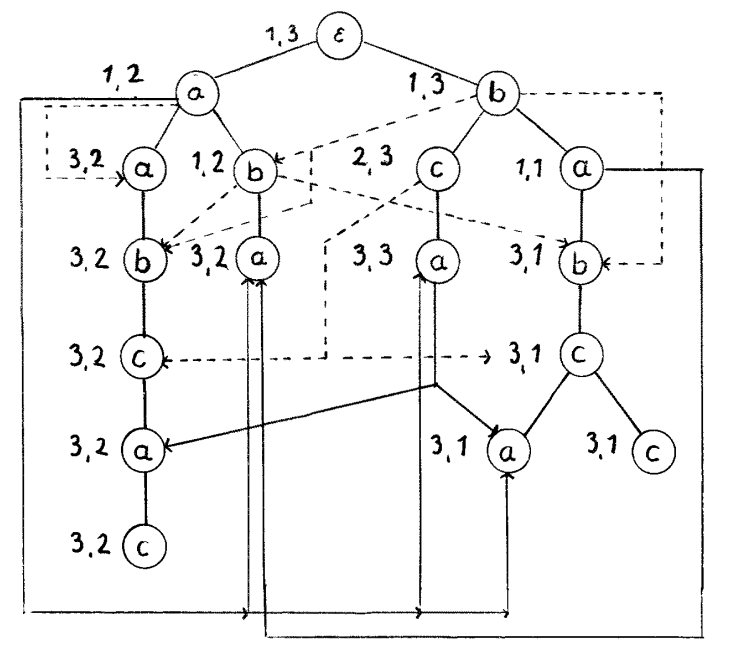
\includegraphics[scale=0.4]{trie.png}
\end{center}

\section{Faza wyszukiwania w tekście}
Wynikiem tej fazy jest lista par postaci $(w, i)$, gdzie $w$ to któryś z szukanym wzorców, natomiast $i$ to pozycja w tekście, na której został znaleziony wzorzec $w$. Faza ta działa następująco. Załóżmy, że mamy już zbudowane drzewo trie składające się z wszystkich wzorców, ale wstawionych do drzewa trie w odwróconej kolejności. Cała sztuczka polega teraz na tym, że dopasowywanie robimy jak w algorytmie Aho-Corasick chodząc po drzewie trie, ale korzystając z pomysłu zapożyczonego z algorytmu Boyera-Moore'a, w przypadku niezgodności znaków używamy funkcji shift1 oraz shift2, aby wykonać odpowiedni skok w tekście, w którym dopasowujemy wzorce z drzewa trie. Zamieszczony poniżej pseudokod dość dokładnie tłumaczy jak wygląda ta kluczowa faza algorytmu.

\begin{algorithm}
\caption{Commentz-Walter, faza wyszukiwania}\label{euclid}
\begin{algorithmic}[1]
\Procedure{Commentz-Walter-search}{$text, n, trie$} \Comment{tekst, długość, drzewo trie wzorców}
\State $v := root(r)$ \Comment{obecnie przetwarzany wierzchołek trie}
\State $i := wmin$ \Comment{obecnie przetwarzana pozycja w tekście}
\State $j := 0$ \Comment{głębokość $v$ w drzewie trie}

\While{ $j \leq n$ }
    \While {$\exists$ dziecko $v'$ wierzchołka $v$ takie, że $l(v')=t[i-j]$} \Comment{faza skanowania}
        \State $v = v'$
        \State $j = j + 1$
        \State \textbf{yield} $(w, i)$ dla każdego $w \in out(v)$
    \EndWhile
\State $shift(v, t[i-j]) := \min(\max(shift1(v), char(t[i-j])-j-1), shift2(v))$
\State $i = i + shift(v, t[i-j])$ \Comment{faza przesuwania tekstu}
\State $j = 0$
\EndWhile
\EndProcedure
\end{algorithmic}
\end{algorithm}

Pozostaje uzasadnić, że ten algorytm na pewno zwraca wszystkie wystąpienia wzorców w tekście. Nie ma wątpliwości co do tego, że każda zwrócona para $(w, i)$ jest na pewno dobrym wystąpieniem. Pozostaje więc się upewnić, że na pewno żadne wystąpienie któregoś z wzorców nie jest pomijane. Z budowy algorytmu wynika, że jedynym podejrzanym miejscem jest moment robienia przesunięcia w tekście. Potrzebujemy, więc podać argument, że $t[i-j+1]\cdots t[i] = w_t^R(v)$ dla pewnego $v \in T$ implikuje, że nie istnieje takie $i'$, że $i < i' < s(v, t[i-j])$ oraz $t[i'-|w|+1]\cdots t[i']$ dla pewnego wzorca $w$. Jednak z definicji $s(v, t[i-j])$ mamy tę własność po prostu za darmo.

\section{Faza przygotowania wzorców}
W tej fazie algorytmu na wejściu mamy zbiór wzorców, a na wyjściu chcemy mieć drzewo trie dla tego zestawu wzorców oraz obliczone dla niego funkcje out, shift1, shift2 oraz char. Chcielibyśmy to wszystko zrobić w czasie liniowym względem sumy długości wzorców. Oczywiście konstrukcja trie w takim czasie jest natychmiastowo. Po prostu dodajemy kolejne słowa budując jednocześnie drzewo. Z definicji funkcji char i out również wynika prostota ich obliczania wprost z definicji. Kłopotliwe mogą się wydawać na pierwszy rzut oka kluczowe funkcje shift1 oraz shift2.

Jednak cały problem mamy już rozwiązany za pomocą algorytmu Aho-Corasick. Mianowicie rozważmy pewną funkcje $f$ zdefiniowaną na wierzchołkach drzewa trie $T$ za pomocą formuły $f(v') = v$, jeżeli $w(v)$ jest maksymalnym sufiksem właściwym $w(v')$ w drzewie $T$. Funkcja ta idealnie współgra z funkcją fail z automatu Aho-Corasick, więc to co musimy zrobić, aby ją obliczyć, to odpalić fazę konstrukcji z algorytmu Aho-Corasick i w czasie jednego przejścia algorytmem bfs po drzewie trie obliczyć funkcję fail. Okazuje się bowiem, że funkcja $set1'$ odwrotna do funkcji $f$, czyli $set1'(v) = \{v' : f(v')=v \}$, to dokładnie podzbiór szukanego przez nas zbioru $set1$, który potrzebujemy do obliczenia funkcji przesunięć. Ponadto zawiera on wierzchołki $v' \in set1(v)$ takie, że $d(v')-d(v)$ jest minimalne. Wynika stąd, że funkcję shift1 można istotnie obliczyć w czasie liniowym. Analogicznie obliczamy funkcję shift2 rozważając zbiór $set2'(v) = \{ v' : v' \in set1'(v), out(v') \not = \emptyset\}$. 

\section{Złożoność obliczeniowa algorytmu}
Faza konstrukcji drzewa trie opisana powyżej jest wykonywana w czasie liniowym względem sumy długości wszystkich wzorców. Przeszukiwanie tekstu pesymistycznie może mieć czas liniowy względem iloczynu długości tekstu, w którym wyszukujemy, z długością najdłuższego wzorca, ale dzięki temu, że mamy funkcje przesunięć, bardzo często nie skanujemy całego tekstu znak po znaku, tylko jego części. Poprzez silną analogię do algorytmu Boyera-Moore'a stwierdzamy, że algorytm Commentz-Walter, działa średnio podobnie jak algorytm Boyera-Moore'a, czyli bardzo szybko. Pesymistycznie jednak pamiętać należy, że może mieć złożoność $O(nm)$, gdzie $n$, to długość tekstu, a $m$ to długość najdłuższego wzorca.
\end{document}